\documentclass[a4paper]{article}
\usepackage{amsmath,amssymb,biblatex,booktabs,caption,enumitem,float,geometry,graphicx,indentfirst,minted,parskip,pdfpages,tabularx,xcolor}
\addbibresource{project.bib}
\captionsetup[figure]{labelsep=period}
% \captionsetup[table]{labelsep=period}
\definecolor{bg}{rgb}{0.95,0.95,0.95}
\geometry{left=3.5cm,right=3.5cm,top=3.3cm,bottom=3.3cm}
\setlength{\parindent}{2em}
\usemintedstyle{emacs}
\begin{document}
\begin{titlepage}
    \vspace*{0.25cm}
    \noindent\rule[0.25\baselineskip]{\textwidth}{1pt}
    \begin{center}
        \huge{\textsc{UM--SJTU Joint Institute}}\vspace{0.3em}\\
        \huge{\textbf{Embedded System Design (VE373)}}\vspace{0.3em}\\
        \Large{(Design of Microprocessor Based Systems)}
        \noindent\rule[0.25\baselineskip]{\textwidth}{1pt}
    \end{center}
    \begin{center}
        \vspace{5cm}
        \Large{\textsc{Project Report}}\vspace{0.5em}\\
        \Large{\textbf{Hand Gesture Controlled Mantis}}\vspace{1em}\\
        \Large{\textbf{Group 8}}\\
    \end{center}
    \vfill
    \large
    \begin{tabular}{ll}
        Name: Yihua Liu \hspace*{2em}&ID: 518021910998\hspace*{2em}\\
        Name: Xingyuan Wang \hspace*{2em}&ID: 518370910198\hspace*{2em}\\
        Name: Haorong Lu \hspace*{2em}&ID: 518370910194\hspace*{2em}\\
        \\
        Date: \today
    \end{tabular}
\end{titlepage}
\tableofcontents
\newpage
\section{Objectives}
\begin{itemize}
    \item Implement a mantis-like robot that can move forward, backward, to the left, and to the right.
    \item Implement remote control for the robot by hand gestures through Bluetooth.
    \item Implement the function of obstacle avoidance for the robot.
\end{itemize}
\section{Introduction}
\subsection{Overview}
In this project, we have designed and implemented a robot which can be controlled remotely using gestures. The robot uses 2 feet with 4 servos to move with another 2 wheels for additional supporting, and has the basic functions including standing, moving forward, moving backward, turning clockwise, and turning counterclockwise. The movement of the robot is controlled by hand gestures using an accelerometer-integrated glove, and the communication between the control side and the robot is established via Bluetoorh modules. Two PIC32 boards are used in the project, with one on the robot controlling the movement of the robot, and the other connected to the glove detecting and sending gesture control signals to the robot. Another additional Arduino board is used for connecting the accelerometer with PIC32 via I2C. A standalone battery and a power management IC is used for the power supply of the 4 servos on the robot, and an ultrasonic distance detector is placed on the robot so that is stops moving forward automatically when there are obstacles in front of it. 
\subsection{Mechanical Structure}
\begin{figure}[H]
    \centering
    \includegraphics[width=0.8\textwidth]{Robot.pdf}
    \caption{Mechanical Structure of the Robot.}
\end{figure}
\subsection{Photos of the Designed System}
\begin{figure}[H]
    \centering
    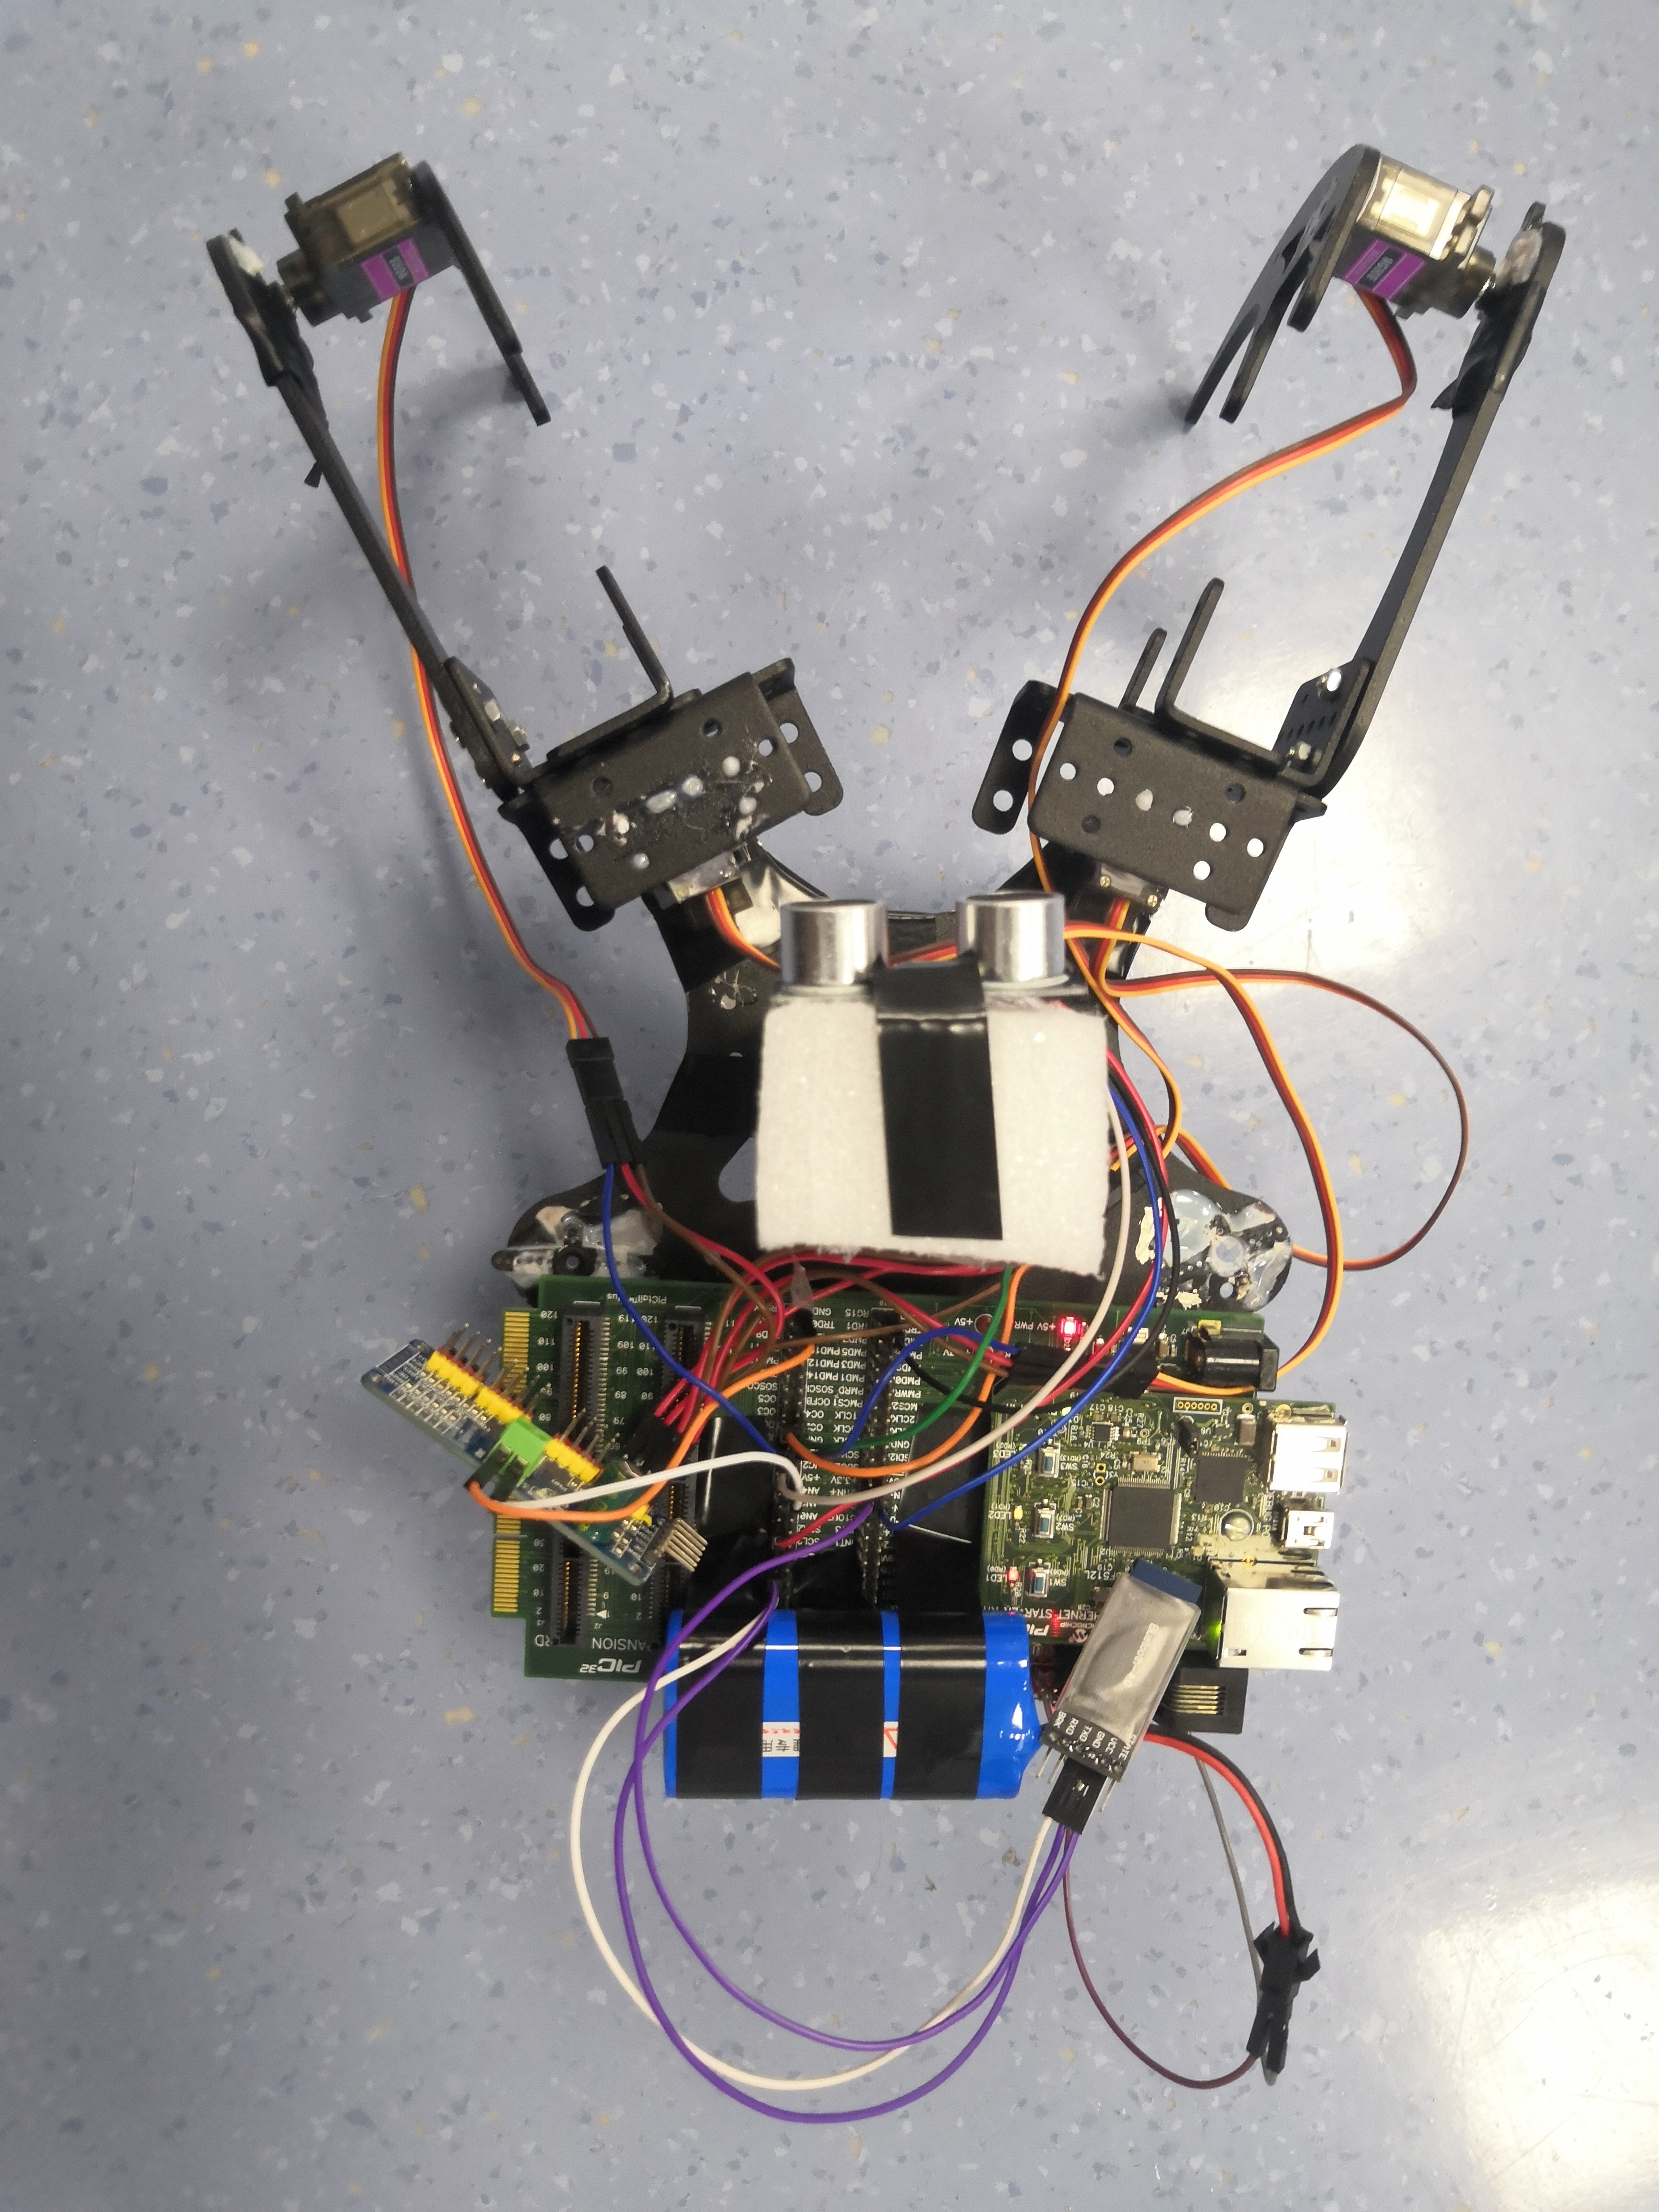
\includegraphics[width=0.6\textwidth]{Top View.jpg}
    \caption{Top View of the Robot.}
\end{figure}
\begin{figure}[H]
    \centering
    \includegraphics[width=0.8\textwidth]{Front View.jpg}
    \caption{Front View of the Robot.}
\end{figure}
\begin{figure}[H]
    \centering
    \includegraphics[width=0.8\textwidth]{Left View.jpg}
    \caption{Left View of the Robot.}
\end{figure}
\begin{figure}[H]
    \centering
    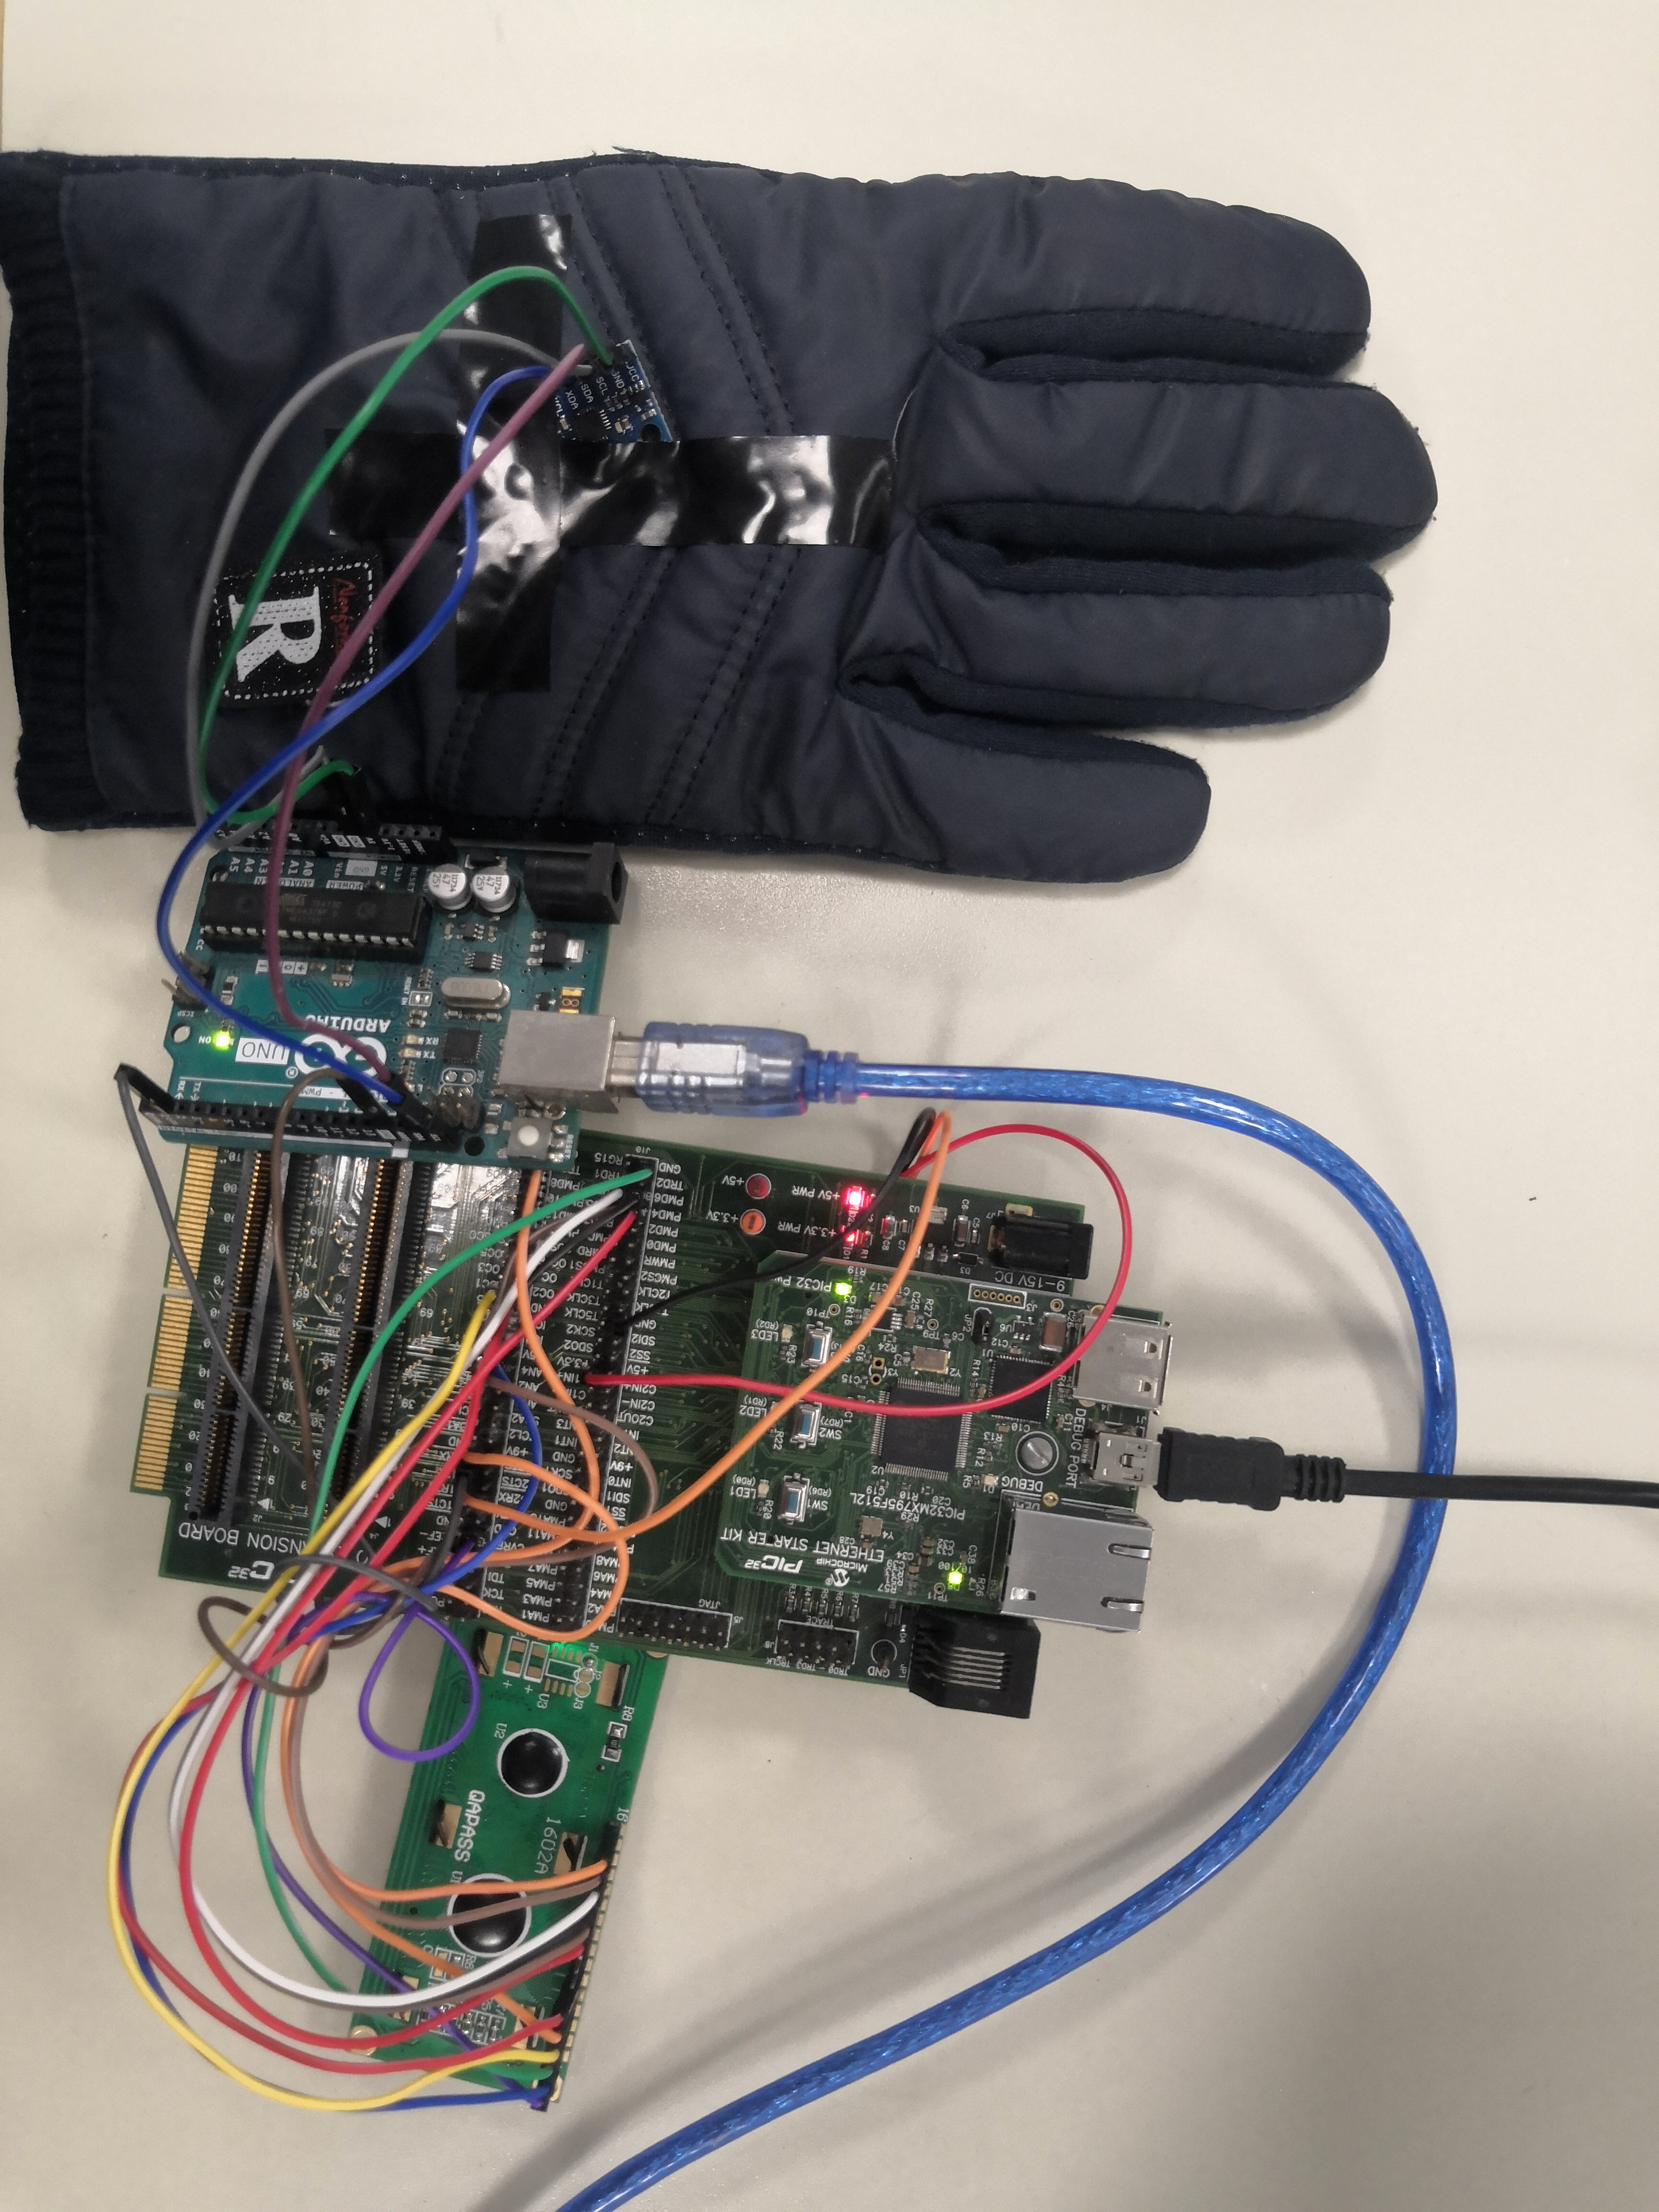
\includegraphics[width=0.6\textwidth]{Circuits.jpg}
    \caption{The Circuits of the Remote Control Part.}
\end{figure}
\subsection{Top-level Block Diagram}
\begin{figure}[H]
    \centering
    \includegraphics[width=0.8\textwidth]{Diagram.pdf}
    \caption{Top-level Block Diagram.}
\end{figure}
\section{Schematics}
\begin{figure}[H]
    \centering
    \includegraphics[width=1\textwidth]{Remote Control Schematic.pdf}
    \caption{Remote Control Schematic\protect\footnotemark[1].}
\end{figure}
\footnotetext[1]{The library of HM-10 BLE Blootooth 4.0 refers to \cite{ADHM10}.}
The original print of the schematic is appended in Appendix.
\section{Component Diagram}
This section covers the main peripheral components used in our project.
\subsection{Motion Tracking Device}
In this project, we use MPU-6050, which is an six DoF accelerometer and gyroscope as our motion tracking device for remote control using hands. It measures temperature, acceleration and gravity data in x, y and z axis directions, and communicates with our microprocessor using I2C protocol. The pins used in our program have been labelled in the following diagram.
\begin{figure}[H]
    \centering
    \includegraphics[width=1\textwidth]{MPU.jpg}
    \caption{Component diagram of MPU-6050.}
\end{figure}

However, after some attempts, we find that the I2C module of the PIC32 board cannot work together with the MPU-6050. Our solution is to use an Arduino Uno board as the "intermediary" between MPU-6050 and the PIC32 board. As shown in the functional block diagram in the previous section, the MPU-6050 communicates with the Arduino Uno board through the I2C protocol, and the Arduino Uno board communicates with the PIC32 board through UART protocol. For the MPU-6050, its VCC pin is connected to the $5V$ output of the Arduino Uno board, and the GND pin is connected to the same ground as Arduino Uno. MPU-6050's SCL and SDA pins are connected to the SCL and SDA pins of the Arduino Uno board. In the I2C communication, the MPU-6050 operates in a slave mode while the Arduino Uno operates in the master mode. The other four pins of MPU-6050 are for auxiliary data, clock, address transportation and interrupt, which are not needed in our case.

For the Arduino Uno board, we connect its $V_{in}$ and GND pins to the $5V$ output and GND pins of the PIC32 board, and its UART Tx pin to the U1RX pin of the PIC32 board, because in our situation, we only a need one-way connection from the Arduino Uno board to the PIC32 board.

\subsection{Bluetooth Module}
We choose the HM-10 Bluetooth module in our project to establish the remote connection between the hand motor detector and the robot. We use the Bluetooth module on the hand motor detector as the transmitter and use the Bluetooth module on the robot as the receiver, with motion instructions being transmitted. Similar to the communication between the Arduino Uno board and the PIC32 board, we only need to implement the one-way communication between the hand motion detector and the robot.

\begin{figure}[H]
    \centering
    \includegraphics[width=1\textwidth]{HM10.jpg}
    \caption{Component diagram of HM-10.}
\end{figure}

The configuration of the Bluetooth modules is done manually. We connect each Bluetooth module to a computer by using a USB to TTL converter and an application which supports serial communication. We send a 'AT+MODE0' message to each Bluetooth module to put them into the data transmission mode. Then we send 'AT+ROLE1' to the Bluetooth module on the hand motion detector to put it into master mode, and send 'AT+ROLE0' to the Bluetooth module on the robot to put it into slave mode. The HM-10 Bluetooth module supports auto-connection, namely a Bluetooth in master mode can automatically detect nearby Bluetooth module that is in slave mode, and connect to it. Therefore, there is no need to setup the connection manually every time, we just need to turn on the power, and the two Bluetooth modules will connect each other automatically.

As only one-way data transmission is used in our project, only 3 pins labelled in the diagram is needed. The Bluetooth module is connected to our PIC32 via UART with a required baud rate being 9600. On the hand motion detector, we connect two pins for power supply, and then connect the UART Rx pin of the Bluetooth module to the U1TX pin of the PIC32 board. On the robot, we also connect two pins for power supply, and then connect the UART Tx pin of the Bluetooth module to the U1RX pin of the PIC32 board. Also, we use DMA to transmit received data to a larger memory space as soon as the receiver has data available.

\subsection{Servo}
In this project, we use 4 servos to control the motion of the 2 front legs of our spider, since each leg needs to move upward, downward, forward and backward. We choose MG90S as our servo, which has a rotating angle between 0 and 180 degrees controlled by PWM signals. The required frequency of the PWM signal is 50Hz. The following diagram shows the pinout of the servo.

\begin{figure}[H]
    \centering
    \includegraphics[width=0.7\textwidth]{servo.jpg}
    \caption{Component diagram of MG90S.}
\end{figure}

As can be seen from the diagram, we need one PWM signal per servo which makes a total of 4 PWM signals. The PIC32 board has five output compare modules OC1-OC5, and that's enough for us to use OC to generate the PWM signals for 4 servos. The relationship between the duty cycle of PWM signal and the degree of servo is shown in the table below.

\begin{table}[htbp]
    \centering
    \begin{tabular}{cc}    
        \toprule    
            Duty Cycle & MG90S Servo Degree \\    
        \midrule
            $2.5\%$   & $0^\circ$       \\
            $5.0\%$   & $45^\circ$       \\
            $7.5\%$   & $90^\circ$       \\
            $10.0\%$   & $135^\circ$       \\
            $12.5\%$   & $180^\circ$       \\
    \end{tabular}
    \caption{Duty Cycle v.s. MG90S Servo Degree}  
\end{table}

Besides the PWM signal generating, another problem is how to power these servos. The Arduino motor shield we used in the lab can only support the power supply for 2 servos. Therefore, we purchase a PCA9685 board that can support the power supply for at most 16 servos. The following diagram shows the appearance of the PCA9685 board.

\begin{figure}[H]
    \centering
    \includegraphics[width=0.7\textwidth]{PCA.png}
    \caption{Appearance of the PCA9685 board.}
\end{figure}

On our robot, we connect the $5V$ output and GND of the PIC32 board to the $V_{in}$ and GND (the green part in the figure above) of the PCA9685, and connect each servo to one pair of the V+ and GND pins (the red and black part) respectively.

\subsection{Distance Detector}
We plan to add an ultrasonic distance sensor HC-SR04 on our spider facing forward which detects the distance between the spider and potential obstruction in its front. The diagram of HC-SR04 is shown below.
\begin{figure}[H]
    \centering
    \includegraphics[width=0.5\textwidth]{SR.jpg}
    \caption{Component diagram of HC-SR04.}
\end{figure}
The GPIO pin of PIC32 connected to TRIG pin in HC-SR04 sends a high value exceeding 10$\mu s$ to trigger the distance measurement. If any signal comes back to the module, the distance will be proportional to time of high value on ECHO pin. In this case, we use an input capture module to measure that time of high value on ECHO pin. When the distance is below a certain value, the spider is expected to refuse moving forward.

\section{Tests and Results}
Our test plan generally has three phases, we first do a single unit test on each component, and then test the hand motion detector and the robot respectively. Finally we connect this two parts together, and test the overall operating status.
\subsection{MPU-6050}
In the program on the Arduino Uno board, we print the data received from MPU-6050, and use Arduino's serial monitor to show the results. It appears that the data we get for each hand motion (stay and flip left/right/forward/backword) confirms to the datasheet description and can be separable.

\subsection{HM-10 Bluetooth Module}
We use USB to TTL converter to connect each HM-10 to one computer, and use serial communication application to control and test the HM-10 modules. We first send 'AT+ROLE0' to one HM-10 and 'AT+ROLE1' to another HM-10, and they both send back 'OK:SET+0/1', which indicates that they have correctly accepted the AT command. Then the red lights on both HM-10 change from flashing to steady, which shows that the auto-connection function of two modules works well. Finally we send a message from one HM-10 to another HM-10 module through the serial communication application, and another HM-10 correctly receives the same message. We can conclude that our Bluetooth module works well.

\subsection{Servo}
We directly connect one servo to the PIC32 board and write a simple program that generates a PWM signal with different duty cycles to test it. It appears that the servo's behavior conforms to the relationship between the duty cycle and servo's degree in the previous section, and it's strong enough to rotate the whole leg.

\subsection{Distance Detector}
The test plan of the distance detector is similar to the test plan of MPU-6050. We connect it to the Arduino Uno board and use the serial monitor to show its result. It appears that the HC-SR04 ultrasonic sensor can reflect properly the changes in the distance between it and the nearest obstacle.

\subsection{Hand Motion Detector}
After testing the MPU-6050 and HM-10, we connect them together to test te whole hand motion detector. We connect an LCD screen to the PIC32 board so that we can check the data it receives. We test five different hand motions, and the result on the LCD and arduino's serial monitor shows that the Arduino Uno board correctly process the raw data from the MPU-6050 and generate the direction, and the PIC32 board can properly receive the direction.

\subsection{Robot}
After we finish the configuration of each servo, assembling the robot, and determining the moving algorithm, we start to test the entire moving function of the robot. The test plan is quite simple, 
we manually set the direction we want the robot to move, and check its behavior. As shown in our video, its moving behavior conforms to our expectation.

\subsection{Overall Test}
Since the hand motion detector and robot work well, we only have to connect them together through Bluetooth, and check the overall behavior. As shown in our video, we can see that the robot moves properly according to our hand motion, and the delay between these two parts is short. In addition, when the distance detector find there is an obstacle close to it, the robot will stop moving forward to protect its legs. Generally, we are satisfied with the performance of our robot.

\section{Final Material List}

\begin{table}[htbp]
    \centering
    \begin{tabular}{ccc}    
        \toprule    
            Part & Part Number & Price (rmb) \\    
        \midrule
            PIC32 Board   (x2)     & PIC32MX795F512L      & N/A    \\
            Accelerometer          & MPU6050 6DOF         & 14     \\
            Bluetooth   Tx/Rx      & HM-10                & 42     \\
            PWM Servo Driver       & PCA9685              & 22    \\
            Micro Servo (x4)       & MG90S                & 42    \\
            Lipo Battery (x2)      & 6.4V 1800mAh         & 70     \\
            Ultrasonic Sensor      & HCSR04               & 6      \\
            Bracket of Robot       & Heaxpod Spyder       & 200    \\
            USB to TTL Converter   & CH340G               & 30     \\
            Small Wheel (x2)       & 65mm diameter        & 5      \\
            Dupont Lines           & N/A                  & 0      \\
        \bottomrule
            Total Price  &  & 431  \\  
    \end{tabular}
    \caption{Final Material List for our Project}  
\end{table}

The final materials we used for the project is shown in Table 2. Compared with our proposal, we significantly reduce the numbers of MG90S servos since we update the mechanical structure. The detailed usages of these materials are introduced in the previous section.

\section{Final Project Timeline}
\begin{figure}[H]
    \centering
    \includegraphics[width=1\textwidth]{Final Timeline.jpg}
    \caption{Gantt Chart for our Project.}
\end{figure}

The final timeline of our project is shown in the figure above. Compared with our proposed timeline, we spent a lot more time on assembling the robot since it's mechanical structure is very complicated, and we have to waste plenty of time on waiting the AB glue to be completely dry. Therefore we update the mechanical structure of the robot by replacing some legs with two wheels, which makes our robot more strong and robust.

Though there were some unexpected difficulties and accidents, we still finished the whole project on August 1st, which gave us some time to prepare for the demonstration (and other courses' final exams).

\section{Completion of Project Requirements}
\begin{itemize}
  \item Timer: We use timer to generate delay in the servo driver, and also help generate PWM signal
  \item Interrupt: We use interrupt from TMR1 to generate delay, and on the PIC32 board for the hand motion detector, we use the DMA interrupt since DMA is used to transfer data sent by the Arduino Uno shield through UART. (The PIC32 board on the robot use polling to deal with the control signal received by the Bluetooth module, since the motion of the robot must be complete to maintain its stability.)
  \item PWM: We use PWM signal generated by OC1-OC4 to control 4 servos.
  \item ADC: Not used in our project.
  \item Serial communication module: We use I2C to support the communication between Arduino Uno and the MPU-6050, and use UART to support the communication between Arduino Uno and PIC32  board, and the communication between PIC32 board and the Bluetooth module.
  \item DMA: We use DMA on the robot to transmit the received control signals to a larger array, and then we can use some algorithm to find the majority of the control signal sequence.
\end{itemize}
\printbibliography
\section*{Appendix}
\subsection*{Code for Remote Control}
\subsubsection*{Arduino Uno}
\inputminted[frame=single,bgcolor=bg,breaklines,breakanywhere]{arduino}{"main.ino"}
\inputminted[frame=single,bgcolor=bg,breaklines,breakanywhere]{c}{"MPU6050.h"}
\inputminted[frame=single,bgcolor=bg,breaklines,breakanywhere]{c}{"MPU6050.cpp"}
\subsubsection*{PIC32 with MPU-6050}
\inputminted[frame=single,bgcolor=bg,breaklines,breakanywhere]{c}{"main.c"}
\subsubsection*{LCD}
\inputminted[frame=single,bgcolor=bg,breaklines,breakanywhere]{c}{"LCD.h"}
\subsection*{Code for the Robot}
\subsubsection*{PIC32 with Servos}
\inputminted[frame=single,bgcolor=bg,breaklines,breakanywhere]{c}{"servo.c"}
\subsection*{Schematics (Original Print)}
\includepdf[landscape=true]{Remote Control Schematic.pdf}
\end{document}
